\documentclass[10pt,show notes on second screen]{beamer}

\usepackage{appendixnumberbeamer}
\usepackage[numbers,sort&compress]{natbib}
\usepackage{amsfonts}
\usepackage{amsmath}
\usepackage{mathtools}
\usepackage{amssymb}
\usepackage{mathrsfs}
\usepackage{units}
\usepackage{animate}

% \usetheme[progressbar=frametitle]{metropolis}
\usetheme{metropolis}

% For notes
\usepackage{pgfpages}
\setbeamertemplate{note page}[plain]
\setbeameroption{show notes on second screen=bottom}

\usefonttheme[onlymath]{serif}

% Titles, date, ect.
\title{Solving \texorpdfstring{$\SU(3)$}{SU3} Yang-Mills theory on the lattice: a calculation of selected gauge observables with gradient flow}
\date{\today}
\author{Hans Mathias Mamen Vege}
\institute{University of Oslo}

% Loads command list
% For Feynman slashes
\usepackage{slashed}

\newcommand{\husk}[1]{\color{red}#1\color{black}}
\newcommand{\TODO}[1]{\color{red}#1\color{black}}
\newcommand{\expect}[1]{\left\langle{#1}\right\rangle}
\newcommand{\Tr}{\mathrm{Tr}}
\newcommand{\tr}{\mathrm{tr}}
\newcommand{\dd}{\mathrm{d}}
\newcommand{\e}{\mathrm{e}}
\newcommand{\SU}{\mathrm{SU}}
\newcommand{\conj}[1]{\overline{#1}}
\newcommand{\sign}{\mathrm{sign}}
\newcommand{\epsrnd}{\varepsilon_\mathrm{rnd}}

% For fermi units
\newcommand{\fm}{\mathrm{fm}}

% Complex number notation
\renewcommand{\Re}{\operatorname{Re}}
\renewcommand{\Im}{\operatorname{Im}}

% Commands for writing shorthand lattice operators
\newcommand{\MU}{\hat{\mu}}
\newcommand{\NU}{\hat{\nu}}

\renewcommand{\vec}[1]{\boldsymbol{\mathbf{#1}}}
% BEGIN COMMANDS FROM LATEX FOR PHYSICISTS
% http://www.dfcd.net/articles/latex/latex.html
\newcommand{\ket}[1]{\left| #1 \right\rangle} % for Dirac bras
\newcommand{\bra}[1]{\left\langle #1 \right|} % for Dirac kets
\newcommand{\bket}[1]{\right| #1 \right\rangle} % for Dirac bras
\newcommand{\bbra}[1]{\left\langle #1 \left|} % for Dirac kets

% Front page
\setbeamertemplate{title page}{
    \begin{minipage}[c][\paperheight]{\textwidth}
        \ifx\inserttitlegraphic\@empty\else\usebeamertemplate*{title graphic}\fi
        \vfill%
        {
        \centering
        \ifx\inserttitle\@empty\else\usebeamertemplate*{title}\fi
        \ifx\insertsubtitle\@empty\else\usebeamertemplate*{subtitle}\fi
        }
        \usebeamertemplate*{title separator}
        \begin{minipage}[t]{.4\textwidth}
            \ifx\beamer@shortauthor\@empty\else\usebeamertemplate*{author}\fi
            \ifx\insertdate\@empty\else\usebeamertemplate*{date}\fi
        \end{minipage}
        \begin{minipage}[t]{.6\textwidth}
            \vspace*{2em}
            {\hspace{1.2em}\small Supervisor: \textit{Andrea Shindler} \par}
            \vspace*{0.2em}
            {\hspace{1.2em}\small Co-supervisor: \textit{Morten Hjorth-Jensen}}
        \end{minipage}%

        \begin{minipage}[t]{\textwidth}
            \centering
            \ifx\insertinstitute\@empty\else\usebeamertemplate*{institute}\fi
        \end{minipage}
        \vfill
        \vspace*{1mm}
    \end{minipage}
}



\newcommand{\CC}{C\nolinebreak\hspace{-.05em}\raisebox{.4ex}{\tiny\bf +}\nolinebreak\hspace{-.10em}\raisebox{.4ex}{\tiny\bf +}}
\def\CC{{C\nolinebreak[4]\hspace{-.05em}\raisebox{.4ex}{\tiny\bf ++ }}}

% For aligned undersets
\usepackage{stackengine}
\def\stacktype{L}
\setstackgap{L}{1.2\normalbaselineskip}
\stackMath
\tabularnewline

\begin{document}

\setbeamercolor{background canvas}{bg=white}
\maketitle

% \begin{frame}{Structure}
%   % \setbeamertemplate{section in toc}[sections numbered]
%   \tableofcontents[hideallsubsections]
% \end{frame}

\begin{frame}{Structure}
    \begin{itemize}[<+->]
        \item Quantum Chromodynamics(QCD).
        \item Lattice QCD.
        \item Gradient flow.
        \item Developing a code for solving $\SU(3)$ Yang-Mills theory.
        \item Results.
    \end{itemize}
    \note{
    \begin{itemize}[<+->]
        \item \textbf{QCD.} We will go through and explain what QCD as well as motivate its existence.
        \item \textbf{LQCD.} We will briefly show how one discretise the lattice and perform calculations on it.
        \item \textbf{Gradient flow.} We will quickly introduce gradient flow and explain its effects.
        \item \textbf{GLAC.} Will briefly present the code which we developed as well as some benchmarks. We will also present the Metropolis algorithm.
        \item \textbf{Results.} We will present the results obtained from pure gauge calculations.
    \end{itemize}
    }
\end{frame}

%%%%%%%%%%%%%%%%%%%%%%%%%%%%%%%%%%%%%%%%%%%%%%%%%%%%%%%%%%%%%%%%%%%%%%%%%%%%%%%%%%%%%%%%%%
\section{Introduction}
%%%%%%%%%%%%%%%%%%%%%%%%%%%%%%%%%%%%%%%%%%%%%%%%%%%%%%%%%%%%%%%%%%%%%%%%%%%%%%%%%%%%%%%%%%

% \begin{frame}{Motivation}
%     \begin{itemize}[<+->]
%         \item Low-energy regime.
%         \item 
%     \end{itemize}
% \end{frame}

%%%%%%%%%%%%%%%%%%%%%%%%%%%%%%%%%%%%%%%%%%%%%%%%%%%%%%%%%%%%%%%%%%%%%%%%%%%%%%%%%%%%%%%%%%
\section{Quantum Chromodynamics(QCD)}
%%%%%%%%%%%%%%%%%%%%%%%%%%%%%%%%%%%%%%%%%%%%%%%%%%%%%%%%%%%%%%%%%%%%%%%%%%%%%%%%%%%%%%%%%%

\begin{frame}{The standard model}
% Use the nice standard model picture
    \begin{center}
        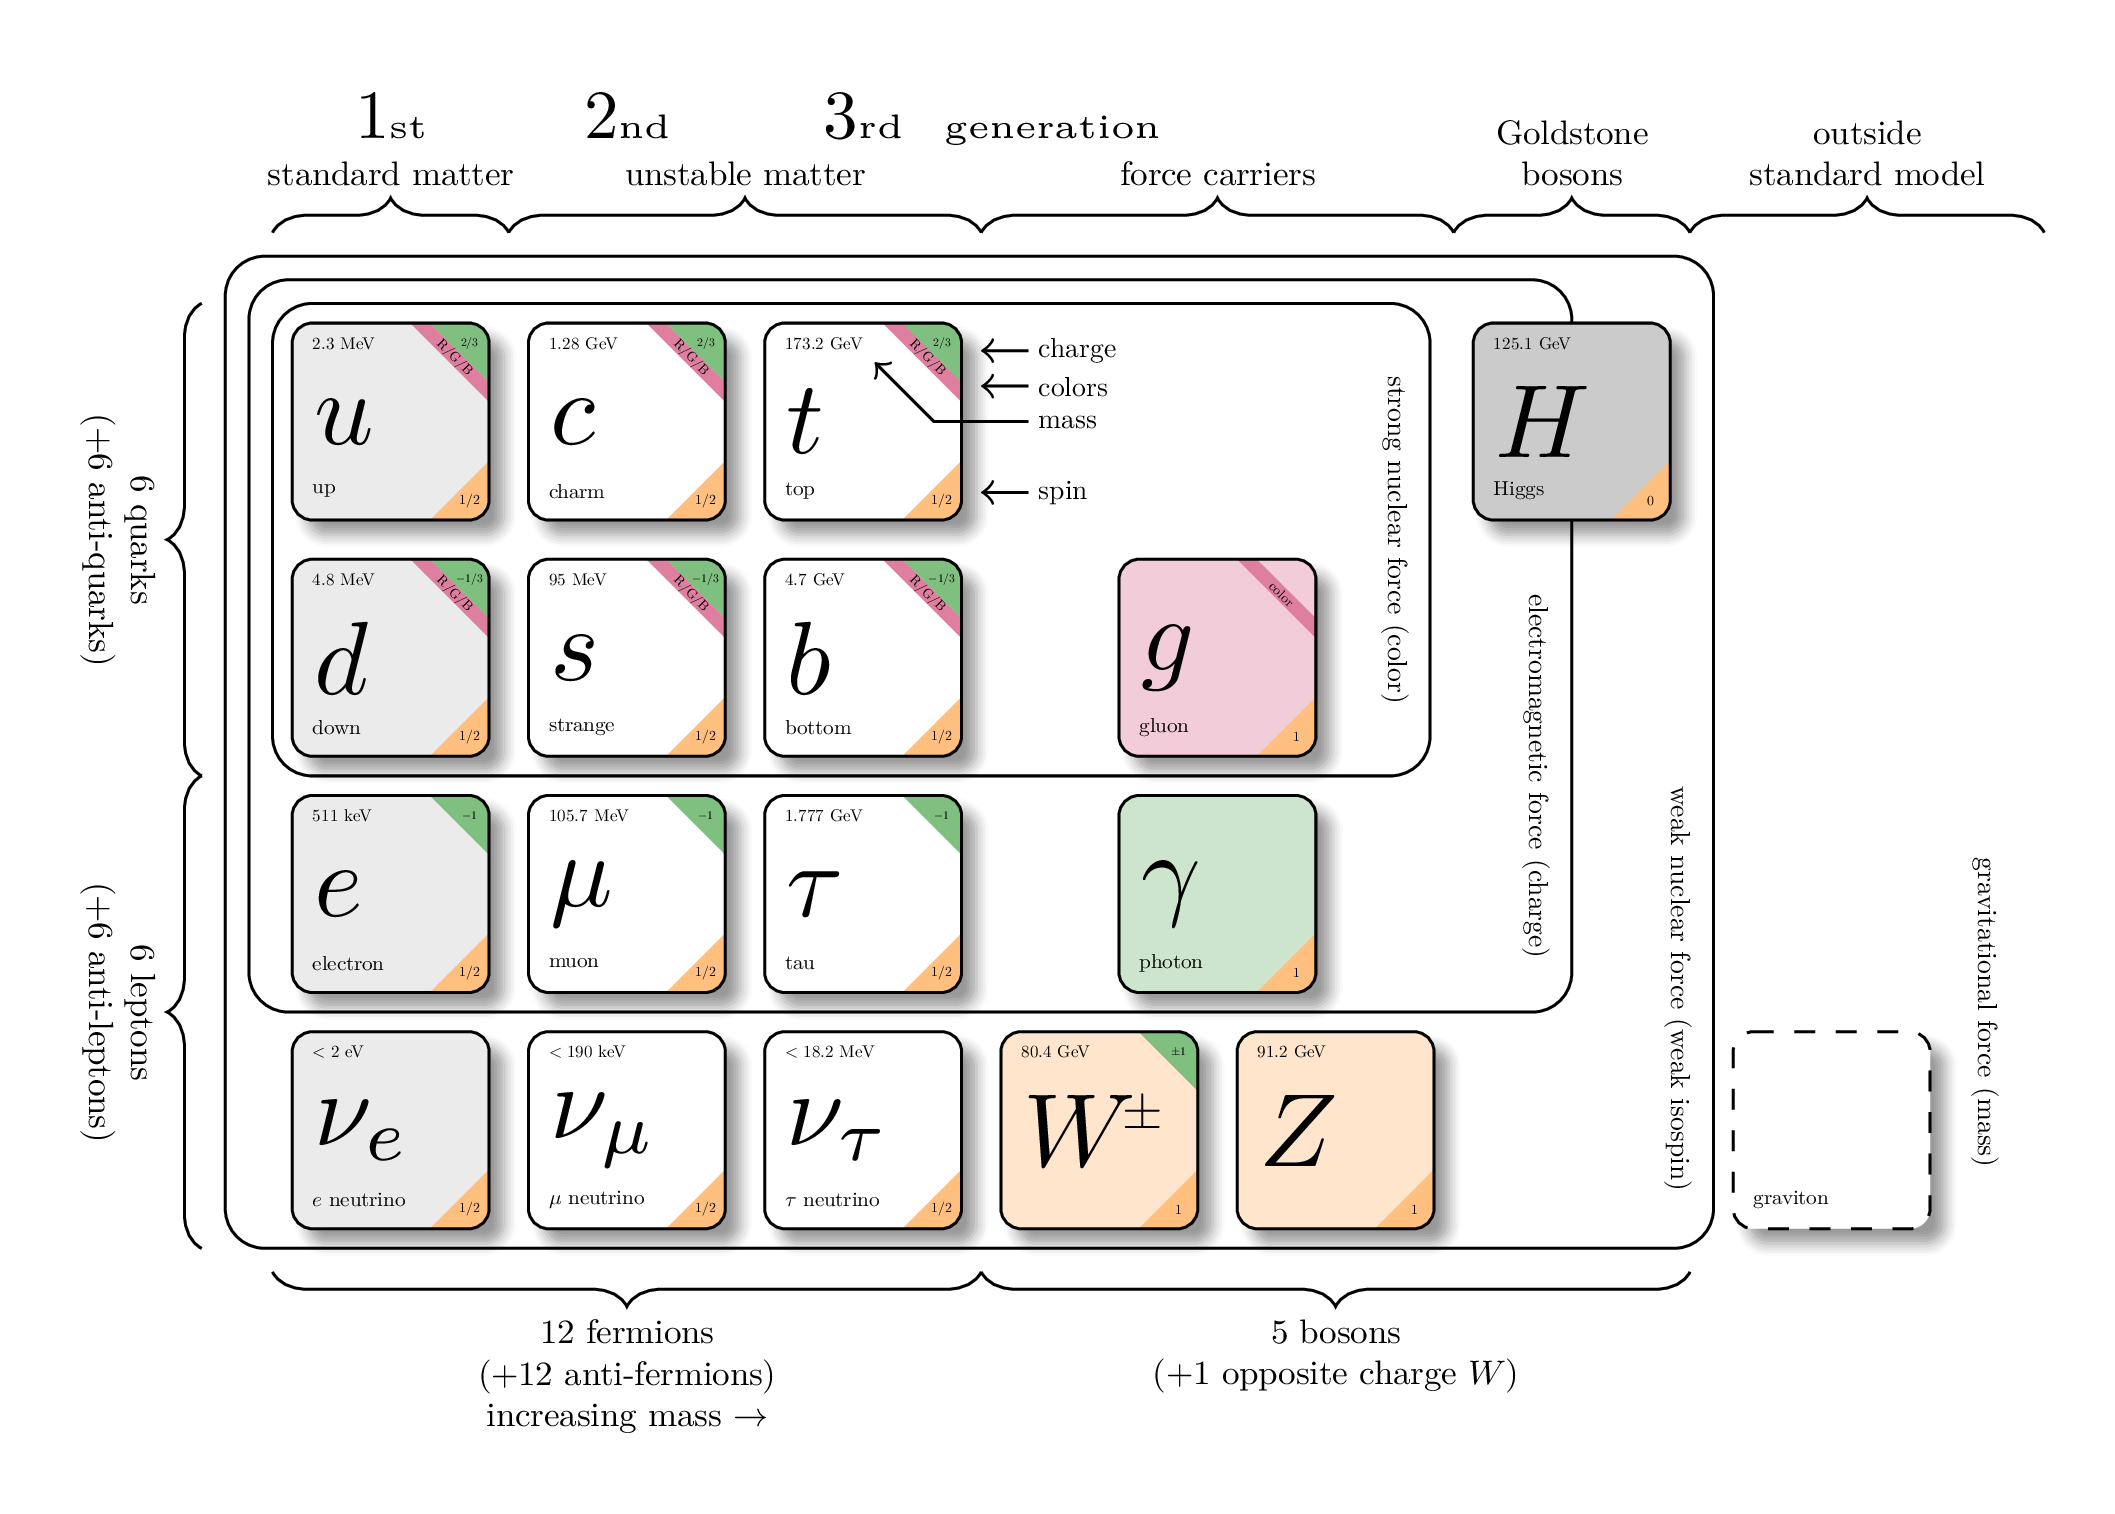
\includegraphics[width=1.0\textwidth]{../figures/illustrations/qcd/standard-model/sm.png}
    \end{center}
    \note{
        \textbf{SM.} A pictorial illustration of the standard model of physics. Lattice QCD is all about exploring the QCD sector consisting of gluons and quarks. We will however focus on the gluons.
    }
\end{frame}


\begin{frame}{QCD}
% Asymptotic freedom
% Confinement
% Experimental proof?
\end{frame}

\begin{frame}{The path integral formalism}
% Simply show how the path integral is written so one has something to relate to
    \begin{itemize}[<+->]
        \item A
    \end{itemize}
\end{frame}

\begin{frame}{Topology in QCD}
    \begin{itemize}[<+->]
        \item A
    \end{itemize}
\end{frame}

\begin{frame}{The Witten-Veneziano relation}
    \begin{itemize}[<+->]
        \item A
    \end{itemize}
\end{frame}

%%%%%%%%%%%%%%%%%%%%%%%%%%%%%%%%%%%%%%%%%%%%%%%%%%%%%%%%%%%%%%%%%%%%%%%%%%%%%%%%%%%%%%%%%%
\section{Lattice Quantum Chromodynamics(LQCD)}
%%%%%%%%%%%%%%%%%%%%%%%%%%%%%%%%%%%%%%%%%%%%%%%%%%%%%%%%%%%%%%%%%%%%%%%%%%%%%%%%%%%%%%%%%%

\begin{frame}{Discretizing spacetime}
    \begin{itemize}[<+->]
        \item A
    \end{itemize}
\end{frame}

\begin{frame}{Links}
\end{frame}

\begin{frame}{Pure gauge action}
\end{frame}

\begin{frame}{Recovering the continuum action action}
\end{frame}

%%%%%%%%%%%%%%%%%%%%%%%%%%%%%%%%%%%%%%%%%%%%%%%%%%%%%%%%%%%%%%%%%%%%%%%%%%%%%%%%%%%%%%%%%%
\section{Developing a code for solving \texorpdfstring{$\SU(3)$}{SU3} Yang-Mills theory on the lattice}
%%%%%%%%%%%%%%%%%%%%%%%%%%%%%%%%%%%%%%%%%%%%%%%%%%%%%%%%%%%%%%%%%%%%%%%%%%%%%%%%%%%%%%%%%%

\begin{frame}{The numerical challenge in lattice QCD}
\end{frame}

\begin{frame}{The path integral}
% Include 
\end{frame}

\begin{frame}{The Metropolis algorithm}
\end{frame}

\begin{frame}{GLAC}
\end{frame}

\begin{frame}{Link sharing}
\end{frame}

\begin{frame}{Shifts}
\end{frame}

\begin{frame}{Scaling}
\end{frame}

%%%%%%%%%%%%%%%%%%%%%%%%%%%%%%%%%%%%%%%%%%%%%%%%%%%%%%%%%%%%%%%%%%%%%%%%%%%%%%%%%%%%%%%%%%
\section{Measuring observables on the lattice}
%%%%%%%%%%%%%%%%%%%%%%%%%%%%%%%%%%%%%%%%%%%%%%%%%%%%%%%%%%%%%%%%%%%%%%%%%%%%%%%%%%%%%%%%%%
\begin{frame}{How to measure}
\end{frame}

\begin{frame}{Topological charge}
\end{frame}

\begin{frame}{Energy}
\end{frame}

%%%%%%%%%%%%%%%%%%%%%%%%%%%%%%%%%%%%%%%%%%%%%%%%%%%%%%%%%%%%%%%%%%%%%%%%%%%%%%%%%%%%%%%%%%
\section{Gradient flow}
%%%%%%%%%%%%%%%%%%%%%%%%%%%%%%%%%%%%%%%%%%%%%%%%%%%%%%%%%%%%%%%%%%%%%%%%%%%%%%%%%%%%%%%%%%

\begin{frame}{The flow equation}
% Bad approx.: diffusion equation
% Topological charge preserved and is more pronounced 
% Why it is needed
% Certain quantities becomes renormalizable
\end{frame}

\begin{frame}{Solving gradient flow on the lattice}
% RK3 classical and then on the lattice
\end{frame}

\begin{frame}{Smearing the lattice}
% LatViz animation
\end{frame}

%%%%%%%%%%%%%%%%%%%%%%%%%%%%%%%%%%%%%%%%%%%%%%%%%%%%%%%%%%%%%%%%%%%%%%%%%%%%%%%%%%%%%%%%%%
\section{Results}
%%%%%%%%%%%%%%%%%%%%%%%%%%%%%%%%%%%%%%%%%%%%%%%%%%%%%%%%%%%%%%%%%%%%%%%%%%%%%%%%%%%%%%%%%%

\begin{frame}{Ensembles}
% Include size and time
\end{frame}

\begin{frame}{Energy and the scale setting}
\end{frame}

\begin{frame}{Topological charge}
\end{frame}

\begin{frame}{Topological susceptibility}
\end{frame}

\begin{frame}{The fourth cumulant}
\end{frame}

\begin{frame}{The topological charge correlator}
\end{frame}

\begin{frame}{The effective glueball mass}
\end{frame}

%%%%%%%%%%%%%%%%%%%%%%%%%%%%%%%%%%%%%%%%%%%%%%%%%%%%%%%%%%%%%%%%%%%%%%%%%%%%%%%%%%%%%%%%%%
\section{Conclusion}
%%%%%%%%%%%%%%%%%%%%%%%%%%%%%%%%%%%%%%%%%%%%%%%%%%%%%%%%%%%%%%%%%%%%%%%%%%%%%%%%%%%%%%%%%%
\begin{frame}
\end{frame}

\begin{frame}
Questions?
\end{frame}


%%%%%%%%%%%%%%%%%%%%%%%% Disposition %%%%%%%%%%%%%%%%%%%%%%%%
% Introduction/overview of presentation: motivation, goal of thesis
% QCD: what is qcd, qcd to pure gauge(max 2 slides), topology quickstart
% LQCD: discretize lattice, links, introduce topological charge with clover, energy
% Flow: introduce gradient flow, motivate
% Latviz animation of Q in flow time and Euclidean time
% Results: energy scale setting, topological charge, distributions, why D1 and D2 differs, top.sus., N_F, eff.mass, 
% Conclusion: 
% Questions?
% Extra slides

\end{document}